\documentclass[main]{subfiles}

\begin{document}

\chapter{Category theory}

\begin{center}
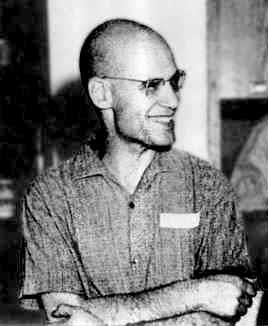
\includegraphics[width=0.5\textwidth]{MyMathematicalUniverse/Pictures/Alexander_Grothendieck.jpg}
\end{center}
\newpage

\tableofcontents
\newpage

\section{Category}

\begin{definition}
A \textit{semicategory}\index{semicategory} $\mathscr C$ consists of
\begin{itemize}
\item A class of \textit{objects}\index{Object} $\Ob\mathscr C$
\item A class of \textit{morphisms}\index{Morphism} $\Hom\mathscr C$
\item Compositions $\Hom(A,B)\times\Hom(B,C)\to\Hom(A,C)$
\end{itemize}
Such that
\begin{itemize}
\item Compositions are associative: $(hg)f=h(gf)$
\end{itemize}
\end{definition}

\begin{definition}
The \textit{empty category}\index{Empty category} is the category without any objects nor morphisms
\end{definition}

\begin{definition}
A \textit{category}\index{Categroy} $\mathscr{C}$ consists of
\begin{itemize}
\item A class of \textit{objects}\index{Object} $\Ob\mathscr C$
\item A class of \textit{morphisms}\index{Morphism} $\Hom\mathscr C$
\item Compositions $\Hom(A,B)\times\Hom(B,C)\to\Hom(A,C)$
\end{itemize}
Such that
\begin{itemize}
\item Compositions are associative: $(hg)f=h(gf)$
\item $\Hom(A,A)$ contains \textit{identity} $1_A$: $1_Af=f$, $g1_A=g$
\end{itemize}
\end{definition}

\begin{definition}
A \textit{subcategory} $\mathscr S$ is a category consists of subclasses of objects and morphisms with the same composition map
\end{definition}

\begin{definition}
The \textit{dual category}\index{Dual category} $\mathscr{C}^{op}$ of $\mathscr{C}$ consists of the same objects and morphisms but with morphisms reversed
\end{definition}

\begin{definition}
A \textit{functor}\index{Functor} $F:\mathscr{C}\to\mathscr{D}$ consists of maps
\begin{itemize}
\item $\Ob\mathscr C\to\Ob\mathscr D$
\item $\Hom_{\mathscr{C}}(A,B)\to\Hom_{\mathscr{D}}(F(A),F(B))$
\end{itemize}
Such that it
\begin{itemize}
\item Preserves identities: $F(1_A)=1_{F(A)}$
\item Preserves compositions: $F(g\circ f)=F(g)\circ F(f)$
\end{itemize}
\end{definition}

\begin{definition}
A \textit{contravariant functor}\index{Contravariant functor} $F:\mathscr C\to\mathscr D$ consists of maps
\begin{itemize}
\item $\Ob\mathscr{C}\to\Ob\mathscr{D}$
\item $\Hom_{\mathscr{C}}(A,B)\to\Hom_{\mathscr{D}}(F(B),F(A))$
\end{itemize}
Such that
\begin{itemize}
\item $F(1_A)=1_{F(A)}$
\item $F(g\circ f)=F(f)\circ F(g)$
\end{itemize}
\end{definition}

\begin{remark}
A contravariant functor $F:\mathscr C\to\mathscr D$ is a functor $F:\mathscr C^{op}\to\mathscr D$
\end{remark}

\begin{definition}
$A\xrightarrow{f}B$ is a
\begin{itemize}
\item \textit{monomorphism}\index{Monomorphism} if $fg_1=fg_2\Rightarrow g_1=g_2$
\item \textit{epimorphism}\index{Epimorphism} if $g_1f=g_2f\Rightarrow g_1=g_2$
\item \textit{bimorphism}\index{Bimorphism} if it is both a monomorphism and an epimorphism
\item \textit{isomorphism}\index{Isomorphism} if it is invertible
\item \textit{automorphism}\index{Automorphism} if it is an isomorphism and $B=A$
\item \textit{constant morphism}\index{Constant morphism} if $fg=fh$ for any $g,h$
\item \textit{coconstant morphism} if $gf=hf$ for any $g,h$
\item \textit{zero morphism}\index{Zero morphism} if it is both constant and coconstant
\item \textit{involution}\index{Involution} if $B=A$ and $f^2=1_A$
\end{itemize}
\end{definition}

\begin{remark}
Isomorphisms are bimorphisms
\end{remark}

\begin{example}
A bimorphism is not necessary an isomorphism. In the category of rings, $\mathbb Z\hookrightarrow\mathbb Q$ is a bimorphism because $\mathbb Q=\mathbb Z_{(0)}$ is a localization and the universal property of localization
\end{example}

\begin{definition}
A \textit{natural transformation}\index{Natural transformation} is a family of morphisms $\eta_A:F(A)\to G(A)$ making the following diagram commute
\begin{center}
\begin{tikzcd}
F(A) \arrow[d, "\eta_A"] \arrow[r, "F(f)"] & F(B) \arrow[d, "\eta_B"] \\
G(A) \arrow[r, "G(f)"]                     & G(B)                    
\end{tikzcd}
\end{center}
For contravariant functors
\begin{center}
\begin{tikzcd}
F(B) \arrow[d, "\eta_B"] \arrow[r, "F(f)"] & F(A) \arrow[d, "\eta_A"] \\
G(B) \arrow[r, "G(f)"]                     & G(A)                    
\end{tikzcd}
\end{center}
$\eta$ is a \textit{natural isomorphism}\index{Natural isomorphism} if $\eta_A$ are isomorphisms
\end{definition}

\begin{definition}
A category $\mathscr C$ is 
\begin{itemize}
\item \textit{small}\index{Small category} if $ob(\mathscr C)$ and $\Hom(\mathscr C)$ are sets
\item \textit{locally small}\index{Locally small category} if $\Hom(a,b)$ are sets
\item \textbf{filtered}\index{Filtered category} if it is not empty, and for any two objects $j,j'\in J$, there is an object $k\in J$ and morphisms $f:j\to k$ and $f':j'\to k$, for any two morphisms $u,v:i\to j$, there is an object $k\in J$ and a morphism $w:j\to k$ such that $w\circ u=w\circ v$ \par
A filtered colimit\index{Filtered colimit} is the colimit of a functor $F:J\to\mathscr C$ where $J$ is a filtered category, direct limit is a special case of a filtered colimit \par
The dual notion is called \textbf{cofiltered}
\item \textit{pointed}\index{Pointed category} is a category with zero object
\textit{connected}\index{Connected category} if there is a finite sequence of morphisms connecting any two objects
\end{itemize}
\end{definition}

\begin{example}
$C\leftarrow A\to B$ is a connected even there is no morphism between $B,C$
\end{example}

\begin{definition}
we say categories $\mathscr C,\mathscr D$ are \textit{isomorphic}\index{Isomorphic category} if there are functors $F:\mathscr C\to\mathscr D$ and $G:\mathscr D\to\mathscr C$ such that $G\circ F=1_\mathscr{C}$, $F\circ G=1_\mathscr{D}$ and we say $\mathscr C,\mathscr D$ are \textit{equivalent}\index{Equivalent category} if $G\circ F$ is naturally isomorphic to $1_\mathscr{C}$ and $F\circ G$ is naturally isomorphic to $1_\mathscr{D}$
\end{definition}

\begin{definition}
Suppose $\mathscr C,\mathscr D$ are categories, define the \textit{functor category}\index{Functor category} $[\mathscr C,\mathscr D]$ or $\mathscr D^{\mathscr C}$ has all functors from $\mathscr C$ to $\mathscr D$ as objects, and natural transformations as morphisms
\end{definition}

\begin{definition}
$\mathscr C\times\mathscr D$  is the \textit{product category}\index{Product category} with $ob(\mathscr C\times\mathscr D)=ob\mathscr C\times ob\mathscr D$, $Hom_{\mathscr C\times\mathscr D}(A\times B,C\times D)=Hom_{\mathscr C}(A,C)\times Hom_{\mathscr D}(B,D)$
\end{definition}

\begin{definition}
A functor $F:\mathscr C\to\mathscr D$ is
\begin{itemize}
\item \textit{faithful}\index{Faithful functor} if $\Hom_{\mathscr C}(X,Y)\to \Hom_{\mathscr D}(F(X),F(Y))$ is injective
\item \textit{full}\index{Full functor} if $\Hom_{\mathscr C}(X,Y)\to \Hom_{\mathscr D}(F(X),F(Y))$ is surjective
\item \textit{fully faithful} if $\Hom_{\mathscr C}(X,Y)\to \Hom_{\mathscr D}(F(X),F(Y))$ is bijective
\item \textit{essentially surjective}\index{Essentially surjective} if $\forall d\in ob\mathscr D$, $\exists c\in ob\mathscr C$ such that $Fc\cong d$
\end{itemize}
\end{definition}

\begin{theorem}\label{A functor F is an equivalence iff it is fully faithful and essentially surjective}
$F:\mathscr C\to\mathscr D$ is an equivalence iff $F$ is fully faithful and essentially surjective
\end{theorem}

\begin{proof}
If $F$ is an equivalence, there exist functor $G:\mathscr D\to \mathscr C$ and natural isomorphisms $\eta:1_{\mathscr C}\to GF$,  $\xi:1_{\mathscr D}\to FG$, $\forall d\in\mathscr C$, $\xi_d:d=1_{\mathscr D}(d)\to FG(d)=F(Gd)$ is an isomorphism, i.e. $F$ is essentially surjective, similarly, so is $G$ \par
The composition of 
\[Hom(c,c')\xrightarrow{F} Hom(Fc,Fc')\xrightarrow{G} Hom(GFc,GFc'),\quad f\mapsto Ff\mapsto GFf\]
Is the same as
\[Hom(c,c')\xrightarrow{\eta} Hom(GFc,GFc'),\quad f\mapsto\eta_{c}'f\eta_c^{-1}\]
By Exercise \ref{X1,X2 iso and Y1,Y2 iso implies Hom(X1,Y1),Hom(X2,Y2) iso}, this is bijective, thus $Hom(c,c')\xrightarrow{F} Hom(Fc,Fc')$ is injective, i.e. $F$ is faithful. Similarly, consider the composition
\[Hom(Fc,Fc')\xrightarrow{G} Hom(GFc,GFc')\xrightarrow{F} Hom(FGFc,FGFc')\]
We know $Hom(GFc,GFc')\xrightarrow{F} Hom(FGFc,FGFc')$ is surjective, but we also have the following diagram
\begin{center}
\begin{tikzcd}
{Hom(c,c')} \arrow[r, "F"] \arrow[d, "\eta"'] & {Hom(Fc,Fc')} \arrow[d, "\xi"] \\
{Hom(GFc,GFc')} \arrow[r, "F"]                & {Hom(FGFc,FGFc')}             
\end{tikzcd}
\end{center}
Since $\eta,\xi$ are bijective, $Hom(c,c')\xrightarrow{F} Hom(Fc,Fc')$ is surjective, i.e. $F$ is full \par
Conversely, suppose $F$ is fully faithful and essentially surjective, then for any $d\in\mathscr D$, there exists $c$ and an isomorphism $d\xrightarrow{\xi_d} Fc$, denote this $c$ as $Gd$, we can define a functor $G:\mathscr D\to\mathscr C$, $d\mapsto Gd$(Here we have used the axiom of choice), $d\xrightarrow{f}d'\mapsto c\xrightarrow{Gf}c'$ where $FGf=\xi_d^{-1}f\xi_{d'}$ since $F$ is fully faithful
\begin{center}
\begin{tikzcd}
d \arrow[d, "\xi_d"'] \arrow[r, "f"] & d' \arrow[d, "\xi_{d'}"] \\
FGd \arrow[r, "FGf"]                 & FGd'                     \\
Gd \arrow[u, "F"] \arrow[r, "Gf"]    & Gd' \arrow[u, "F"']     
\end{tikzcd}
\end{center}
$\xi:1_{\mathscr D}\to FG$ is a natural isomorphism \par
Since $F$ is fully faithful, there are unique $\eta_c:c\to GFc$, $F(\eta_c)=\xi_{Fc}$ \par
If $f,g:c\to c'$ such that $\eta_{c'}f=\eta_{c'}g$, then $\xi_{Fc'}Ff=\xi_{Fc'}Fg\Rightarrow Ff=Fg\Rightarrow f=g$ \par
If $f,g:c\to c'$ such that $f\eta_{c}=g\eta_{c}$, then $Ff\xi_{Fc}=Fg\xi_{Fc}\Rightarrow Ff=Fg\Rightarrow f=g$
\begin{center}
\begin{tikzcd}
c \arrow[d] \arrow[r] \arrow[dd, "\eta_{c}"', bend right=49]        & c' \arrow[d] \arrow[dd, "\eta_{c'}", bend left=49]       \\
Fc \arrow[d, "G"'] \arrow[r] \arrow[dd, "\xi_{Fc}"', bend right=49] & Fc' \arrow[d, "G"] \arrow[dd, "\xi_{Fc'}", bend left=49] \\
GFc \arrow[d, "F"'] \arrow[r]                                       & GFc' \arrow[d, "F"]                                      \\
FGFc \arrow[r]                                                      & FGFc'                                                   
\end{tikzcd}
\end{center}
$\eta:1_{\mathscr C}\to GF$ is a natural isomorphism
\end{proof}

\begin{definition}
Suppose $u:S\to A$, $v:T\to A$ are morphisms, $v$ filter through $s$ means there is a morphism $w:T\to S$ such that $v=u\circ w$, then mutually filter defines an equivalence relation on monomorphisms(or equivalent by saying that $w$ is an isomorphism), the equivalence classes are called \textit{subobjects}\index{Subobject} of $A$, the dual notion is called \textit{quotient objects}\index{Quotient object}
\end{definition}

\begin{proposition}
Direct limit is an exact functor
\end{proposition}

\begin{definition}
An object $X$ is a
\begin{itemize}
\item \textit{injective object}\index{Injective object} if for any monomorphism $f:Y\to Z$ and morphism $g:Y\to X$, there is a morphism $h:Z\to X$ such that $g=h\circ f$
\begin{center}
\begin{tikzcd}
Y \arrow[r, "f", hook] \arrow[d, "g"] & Z \arrow[ld, "\exists h", dashed] \\
X                                              &                                  
\end{tikzcd}
\end{center}
\item \textit{projective object}\index{Projective object} if for any epimorphism $f:Y\to Z$, and morphism $g:X\to Z$, there is a morphism $h:X\to Y$ such that $g=f\circ h$
\begin{center}
\begin{tikzcd}
                 & X \arrow[d, "g"] \arrow[ld, "\exists h"', dashed] \\
Y \arrow[r, "f", two heads] & Z
\end{tikzcd}
\end{center}
\end{itemize}
\item \textit{initial object}\index{Initial object} if for every $Y$, there is a unique $X\to Y$
\item \textit{final object}\index{Final object} if for every $Y$, there is a unique $Y\to X$
\item \textit{zero object}\index{Zero object} is an object which is both initial and final
\end{definition}

\begin{remark}
Final objects are also called terminal
\end{remark}

\begin{lemma}[Yoneda lemma]\label{Yoneda lemma}\index{Yoneda lemma}
$\mathscr C$ is locally small
\[\Hom(\Hom(c,-),F)\xrightarrow{\cong} F(c), \eta\mapsto\eta_c(1_c)\]
\[\Hom(\Hom(-,c),F)\xrightarrow{\cong} F(c), \eta\mapsto\eta_c(1_c)\]
If $F=\Hom(-,d)$ or $\Hom(d,-)$, then
\[\Hom(\Hom(c,-),\Hom(d,-))\xrightarrow{\cong}\Hom(d,c)\]
\[\Hom(\Hom(-,c),\Hom(-,d))\xrightarrow{\cong}\Hom(c,d)\]
$\Hom(c,-), \Hom(-,c)$ give fully faithful embeddings
\end{lemma}

\begin{proof}\hfill \\
\begin{center}
\begin{tikzcd}
{\Hom(c,c)} \arrow[rrr, "f"] \arrow[ddd, "\eta_c"'] & && {\Hom(c,x)} \arrow[ddd, "\eta_x"] \\
& 1_c \arrow[r, maps to] \arrow[d, maps to] & f \arrow[d, maps to] & \\
& u \arrow[r, maps to]& Ff(u)=\eta_x(f)& \\
F(c) \arrow[rrr, "Ff"']& & & F(x)
\end{tikzcd}
\end{center}
The natural transformation $\eta$ is determined by the element $u$ in $F(c)$
\end{proof}

\begin{remark}
Functor $\Hom(c,-), \Hom(-,c)$ is called \textbf{Yoneda embedding}, here embedding in the sense of a fully faithful functor, which is injective on objects up to isomorphism as in Lemma \ref{Fully faithfull functor is injective on objects up to isomorphism}
\end{remark}

\begin{definition}
A functor $F:\mathscr C\to Set$ is called a \textit{representable} functor if there is an object $A$ in $\mathscr C$ such that $Hom(A,-), F$ are naturally isomorphic, By Yoneda lemma, the isomorphism is determined by an element $a\in A$ called the universal element
\end{definition}

\begin{definition}
Let $\mathscr C$ be a category, we can define \textit{quotient category}\index{quotient category} by moding out a congruence relation $\sim$, here $\sim$ is an equivalence relation on $Hom(X,Y)$ for any $X,Y$ and it respects composition, i.e. suppose $f_1\sim f_2:X\to Y$, $g_1\sim g_2:Y\to Z$, then $g_1\circ f_1\sim g_2\circ f_2$, thus $Hom_{\mathscr C/\sim}(X,Y)=Hom_{\mathscr C}(X,Y)/\sim$
\end{definition}

\begin{definition}
$\mathscr C$ is \textit{concretizable}\index{Concrete category} if there is a faithful functor $F:\mathscr C\to Set$. A morphism $f:X\to Y$ is an \textit{embedding} if $F(f)$ is injective, and for any $F(Z)\xrightarrow{\phi} F(X)$, $Z\xrightarrow{h} Y$ such that $F(Z)\xrightarrow{F(h)} F(Y)$, $F(h)=F(f)\circ\phi$,  $\phi=F(g)$ for some $Z\xrightarrow{g} X$
\end{definition}

\begin{note}
$\mathscr C$ may have different concretization
\end{note}

\begin{definition}
$W$ is a class of morphisms of $\mathscr C$, the \textit{localization}\index{Localization of a category} of $\mathscr C$ with respect to $W$, denoted $\mathscr C[W^{-1}]$, satisfies universal property
\begin{itemize}
\item Any functor $F:\mathscr C\to\mathscr D$ sending morphisms in $W$ to isomorphisms in $\mathscr D$ uniquely factors through the \textit{localization functor} $\mathscr C\to\mathscr C[W^{-1}]$
\end{itemize}
\end{definition}

\begin{construction}
Add formal inverses of the morphisms in $\overline W$
\end{construction}

\begin{note}
$\Hom_{\mathscr C[W^{-1}]}(A,B)$ consists of \textit{roofs} $A\leftarrow C\to B$ and $A\to D\leftarrow B$
\end{note}

\begin{definition}
A \textbf{diagram}\index{Diagram} is a functor $D:J\to \mathscr C$, $J$ is called the \textbf{indexed category}\index{Indexed category}, the diagram $D$ can be thought of as indexing a collection of objects and morphisms in $\mathscr C$ patterned on $J$, we say $D$ is a diagram in $\mathscr C$ shaped $J$ \par
Let $F:J\to\mathscr C$ be a diagram in $\mathscr C$, $N$ be an object in $\mathscr C$, then a \textbf{cone}\index{Cone} from $N$ to $F$ is a family of morphisms $\psi_X$ such that the following diagram commutes, a \textbf{cocone}\index{Cocone} from $F$ to $N$ is a family of morphisms $\psi_X$ such that the following diagram commutes
\begin{center}
\begin{tikzcd}
                      & N \arrow[ld, "\psi_X"'] \arrow[rd, "\psi_Y"] &      \\
F(X) \arrow[rr, "Ff"] &                                              & F(Y)
\end{tikzcd}
\begin{tikzcd}
                                           & N &                            \\
F(X) \arrow[ru, "\psi_X"] \arrow[rr, "Ff"] &   & F(Y) \arrow[lu, "\psi_Y"']
\end{tikzcd}
\end{center}
A \textbf{limit}\index{Limit} of the diagram $F$ is cone $(L,\phi)$ such that for any other cone $(N,\psi)$ there is a unique $u:N\to L$ such that the following diagram commutes, a \textbf{colimit}\index{Colimit} of the diagram $F$ is cone $(L,\phi)$ such that for any other cone $(N,\psi)$ there is a unique $u:L\to N$ such that the following diagram commutes
\begin{center}
\begin{tikzcd}
                      & N \arrow[ldd, "\psi_X"', bend right] \arrow[rdd, "\psi_Y", bend left] \arrow[d, "\exists_1u", dotted] &      \\
                      & L \arrow[ld, "\phi_X"'] \arrow[rd, "\phi_Y"]                                                          &      \\
F(X) \arrow[rr, "Ff"] &                                                                                                       & F(Y)
\end{tikzcd}
\begin{tikzcd}
                                                                            & N                                  &                                                               \\
                                                                            & L \arrow[u, "\exists_1u"', dotted] &                                                               \\
F(X) \arrow[ru, "\phi_X"] \arrow[rr, "Ff"] \arrow[ruu, "\psi_X", bend left] &                                    & F(Y) \arrow[lu, "\phi_Y"'] \arrow[luu, "\psi_Y"', bend right]
\end{tikzcd}
\end{center}
Limits may also be characterized as terminal objects in the category of cones to $F$, thus unique up to isomorphism, so is colimits, a category contains all limits is called \textbf{complete}\index{Complete}, and is called \textbf{cocomplete}\index{Cocomplete} if containing all colimits \par
The \textbf{equaliser}\index{Equaliser} $Eq(f,g)$ is defined to be the limit of the diagram \begin{tikzcd}
X\arrow[shift left, r, "f"] \arrow[shift right, r, "g"'] &Y
\end{tikzcd}, the \textbf{coequaliser}\index{Coequaliser} is the colimit
\end{definition}

\begin{remark}
Direct limit and inverse limit are defined on directed set, thus limit and colimit are more general
\end{remark}

\begin{definition}
A \textbf{directed set}\index{Directed set} $X$ is a set with a preorder $\leq$ and any pair of elements has an upper bound, i.e., $\forall x,y\in X,\exists z\in X$ such that $x\leq z,y\leq z$
\end{definition}

\begin{definition}
Given a directed set $I$, we can define a \textbf{direct(inductive) system}\index{Direct system}, with modules $A_i$, and functions $f_{ij}:A_i\to A_j$, $f_{ii}=1_{A_i}$, $f_{jk}\circ f_{ij}=f_{ik},i\leq j\leq k$, we can also define an \textbf{inverse system}\index{Inverse system}, with module $A_i$, and functions $f_{ij}:A_j\to A_i$, $f_{ii}=1_{A_i}$, $f_{ij}\circ f_{jk}=f_{ik}$ \par
We can define morphism betweem direct and inverse systems and modules \par
Suppose $A_i$ is a direct system, then a morphism $g_i:A_i\to B$ is such that $g_j\circ f_{ij}=g_i,i\leq j$ or $g_i:B\to A_i$ is such that $g_j=f_{ij}\circ g_i,i\leq j$. Suppose $A_i$ is an inverse system, then a morphism $g_i:A_i\to B$ is such that $g_i\circ f_{ij}=g_j,i\leq j$ or $g_i:B\to A_i$ is such that $g_i=f_{ij}\circ g_j,i\leq j$, 
We can define morphisms between direct and inverse systems \par
Suppose $A_i,B_i$ are both direct systems, a morphism $g_i:A_i\to B_i$ is a family of maps such that $g_j\circ f_{ij}=f_{ij}\circ g_i,i\leq j$. Suppose $A_i,B_i$ are both inverse systems, a morphism $g_i:A_i\to B_i$ is a family of maps such that $g_i\circ f_{ij}=f_{ij}\circ g_j,i\leq j$. 
\end{definition}

\begin{definition}
The \textbf{direct limit}\index{Direct limit} of a direct system is a module $A_\infty$ and morphisms $\iota_i:A_i\to A$ with the universal property: given any morphism $g_i:A_i\to B$, it induces a unique $g_\infty:A_\infty\to B$ such that $g\circ\iota_i=g_i$, there is a concrete construction: define the direct limit $\varinjlim A_i=\displaystyle\bigsqcup_{i\in I}A_i/\sim$, where $a_i\sim a_j, a_i\in A_i,a_j\in A_j$ if there is an upper bound $k$ such that $f_{ik}(a_i)=f_{jk}(a_k)$, or equivalently, $a_i\sim f_{ij}(a_i),i\leq j$
\end{definition}

\begin{definition}
The \textbf{inverse limit}\index{Inverse limit} of an inverse system is a module $A_\infty$ and morphisms $\pi_i:A\to A_i$ with the universal property: given any morphism $g_i:B\to A_i$, it induces a unique $g_\infty:B\to A_\infty$ such that $\pi_i\circ g=g_i$, there is a concrete construction: define the inverse limit $\varprojlim A_i=\displaystyle\left\{(a_i)\in\prod_{i\in I}A_i\middle|a_i=f_{ij}(a_j),i\leq j\right\}$, 
\end{definition}

\begin{remark}
Direct limit and inverse limit are dual to each other in the categorical sense
\end{remark}

\begin{definition}
Product, coproduct
The \textbf{biproducts}\index{Biproduct} $(\bigoplus_iA_i,p_i,\iota_i)$ of $A_i$ is such that $(\bigoplus_iA_i,p_i)$ is the product and $(\bigoplus_iA_i,\iota_i)$ is the coproduct
\end{definition}

\begin{remark}
The initial and final object are the limit and colimit of empty diagram \par
In the category of sets, the initial object is $\varnothing$ and a terminal object is $\{*\}$
\end{remark}

\begin{lemma}
$\Hom(X,-)$ functor takes limits to limits, dually, $\Hom(-,X)$ functor takes colimits to limits
\end{lemma}

\begin{proof}
Consider $Y\xrightarrow{f_i}\Hom(X,X_i)$, we want to define a map $Y\to\Hom(X,\varprojlim X_i)$, for $y\in Y$, $X\xrightarrow{f_i(y)} X_i$ induces $X\xrightarrow g\varprojlim X_i$
\end{proof}

\begin{remark}
In general, $\Hom(X,-)$ functor doesn't take colimits to colimits
\end{remark}

\begin{definition}
A \textit{skeleton of a category}\index{Skeleton of a category} $\mathscr D$ of $\mathscr C$ is a full subcategory such that no two objects in $\mathscr D$ are isomorphic and for every object in $\mathscr C$ is isomorphic to some object in $\mathscr D$, the functor $\mathscr D\hookrightarrow\mathscr C$ is an equivalence of categories
\end{definition}

\begin{definition}
Suppose $\mathscr C$ is a category, a \textit{filtered object}\index{Filtered object} $X$ is an object with a \textit{filtration}\index{Filtration} of $X$, a descending filtration
\[\cdots\to X_{n+1}\to X_n\to X_{n-1}\to\cdots\to X\]
Or an ascending filtration
\[X\to\cdots\to X_{n+1}\to X_n\to X_{n-1}\to\cdots\]
\end{definition}

\begin{definition}
Suppose $\mathscr C$ is a category, $f:X\to Y$ is a morphism, the \textit{image}\index{Image of a morphism} of $f$ is a monomorphism $m:I\to Y$ such that there is a morphism $e:X\to I$ such that the following diagram commutes and satisfies the universal property
\begin{center}
\begin{tikzcd}
X \arrow[rr, "f"] \arrow[rd, "e"] \arrow[rdd, "e'"', bend right] &                                                         & Y \\
                                                                & I \arrow[ru, "m", hook] \arrow[d, "\exists_1v", dashed] &   \\
                                                                & I' \arrow[ruu, "m'"', hook, bend right]                 &  
\end{tikzcd}
\end{center}
\end{definition}

\begin{definition}
A \textit{quiver}\index{Quiver} is a functor from \begin{tikzcd}
\bullet \arrow[r, shift left] \arrow[r, shift right] \arrow[loop, distance=2em, in=215, out=145] & \bullet \arrow[loop, distance=2em, in=35, out=325]
\end{tikzcd} to the category of sets. Equivalently, a directed graph allowing multiple arrows and loops
\end{definition}

\begin{definition}
The \textit{free category}\index{Free category} generated by quiver $Q$ has objects vertices in $Q$ and morphisms paths in $Q$ with empty path the identity
\end{definition}

\begin{definition}
$A\xrightarrow{i}B$ has \textit{left lifting property}\index{Left lifting property} or \textit{LLP} and $X\xrightarrow{p}Y$ has \textit{right lifting property}\index{Right lifting property} or \textit{RLP} for each other in this diagram if
\begin{center}
\begin{tikzcd}
A \arrow[r] \arrow[d, "i"]                            & X \arrow[d, "p"] \\
B \arrow[r] \arrow[ru, "\exists" description, dashed] & Y               
\end{tikzcd}
\end{center}
$i,p$ are \textit{orthogonal} if the lifting is unique
\end{definition}

\begin{definition}
A class of morphisms $\mathbf M$ of $\mathscr C$ satisfies \textit{2 out of 3}\index{2 out of 3} if any two of $f,g,f\circ g$ are in $\mathbf M$, so is the third. $\mathbf M$ is clearly closed under composition \par
A class of \textit{weak equivalences}\index{Weak equivalence} is a class of morphisms $\mathbf W$ containing isomorphisms and satisfies 2 out of 3. The class of isomorphisms $\mathbf I$ is a class of weak equivalences
\end{definition}

\begin{definition}
$G$ is a \textit{group object} in category $\mathcal C$(having finite products, thus terminal object $1$) if there are multiplication $m:G\times G\to G$, identity $e:1\to G$, and inverse $i:G\to G$ satisfying the group law
\begin{enumerate}
\item Associativity \begin{tikzcd}
                                                                 & G\times G \arrow[rd, "m"] &   \\
G\times G\times G \arrow[ru, "m\times1"] \arrow[rd, "1\times m"] &                           & G \\
                                                                 & G\times G \arrow[ru, "m"] &  
\end{tikzcd} commutes
\item Unity 
\begin{tikzcd}
1\times G \arrow[r, "e\times 1"] \arrow[rd, "p_2"] & G\times G \arrow[d, "m"] \\
                                                   & G                       
\end{tikzcd}\quad \begin{tikzcd}
G\times 1 \arrow[r, "1\times e"] \arrow[rd, "p_1"] & G\times G \arrow[d, "m"] \\
                                                   & G                       
\end{tikzcd} commute
\item Invertibility
\begin{tikzcd}
                      &                                                          & G\times G \arrow[rd, "m"] &           \\
G \arrow[r, "\Delta"] & G\times G \arrow[ru, "1\times i"] \arrow[rd, "i\times1"] &                           & G\times G \\
                      &                                                          & G\times G \arrow[ru, "m"] &          
\end{tikzcd} commutes
\end{enumerate}
\end{definition}

\begin{definition}
$Y$ is an object such that all binary products $X\times Y$ exist, the \textbf{exponential object}\index{Exponential object} is $Z^Y$ together with morphism $Z^Y\times Y\xrightarrow{\mathrm{eval}} Z$ satisfying universal property
\begin{center}
\begin{tikzcd}
X\times Y \arrow[rd, "f"] \arrow[d, "\exists_1\tilde f\times1_Y"', dashed] &   \\
Z^Y\times Y \arrow[r, "\mathrm{eval}"']                                    & Z
\end{tikzcd}
\end{center}
\end{definition}

\begin{proposition}
$Hom(X\times Y,Z)\to Hom(X,Z^Y)$ is an adjunction
\end{proposition}

\begin{definition}
Consider functors $S:\mathscr A\to\mathscr C$, $T:\mathscr B\to\mathscr C$(for source and target), define \textbf{comma category}\index{Comma category} $(S\downarrow T)$ with objects $(A,B,h)$, $A\in\mathscr A,B\in\mathscr B$ are objects, $h:S(A)\to T(B)$ is a morphism, and with morphisms $(f,g):(A,B,h)\to(A',B',h')$ where $f:A\to A',g:B\to B'$ are morphisms such that the following diagram commutes
\begin{center}
\begin{tikzcd}
S(A) \arrow[r, "S(f)"] \arrow[d, "h"'] & S(A') \arrow[d, "h'"] \\
T(B) \arrow[r, "T(g)"]                 & T(B')                
\end{tikzcd}
\end{center}
\end{definition}

\begin{definition}
Consider the comma category of $1_{\mathscr A}:\mathscr A\to\mathscr A$, $T:*\to\mathscr A$ which we call \textbf{slice category}\index{Slice category}, sometimes denoted as $(\mathscr A\downarrow A_*)$ where $A_*=T(*)$, the objects of the slice category are $A\xrightarrow{\pi_A}A_*$ and morphisms are
\begin{center}
\begin{tikzcd}
A \arrow[rr, "f"] \arrow[rd, "\pi_A"'] &     & A' \arrow[ld, "\pi_{A'}"] \\
                                       & A_* &                          
\end{tikzcd}
\end{center}
Its dual notion, the comma category of $S:*\to\mathscr B$ $1_{\mathscr B}:\mathscr B\to\mathscr B$, which we call \textbf{coslice category}\index{Coslice category}, sometimes denoted as $(B_*\downarrow\mathscr B)$ where $B_*=S(*)$, the objects of the slice category are $B_*\xrightarrow{\pi_B}B$ and morphisms are
\begin{center}
\begin{tikzcd}
                  & B_* \arrow[ld, "\pi_B"'] \arrow[rd, "\pi_{B'}"] &    \\
B \arrow[rr, "g"] &                                                 & B'
\end{tikzcd}
\end{center}
The comma category of $1_{\mathscr C}:\mathscr C\to\mathscr C$, $1_{\mathscr C}:\mathscr C\to\mathscr C$ which we call \textbf{arrow category}\index{Arrow category}, sometimes denoted as $\mathscr C^{\to}$ the objects of the arrow category are just the morphisms(arrows) $A\xrightarrow{f}A'$, and morphisms are
\begin{center}
\begin{tikzcd}
A \arrow[r, "f"] \arrow[d, "h"'] & A' \arrow[d, "h'"] \\
B \arrow[r, "g"]                 & B'                
\end{tikzcd}
\end{center}
\end{definition}

\begin{definition}
A right inverse are called a \textbf{section}\index{Section}, a left inverse is called a \textbf{retraction}\index{Retraction}
\begin{center}
\begin{tikzcd}
X \arrow[rd, equal] \arrow[r, "f"] & Y \arrow[d, "g"] \\
                            & X               
\end{tikzcd}
\end{center}
$f$ is a section of $g$, $g$ is a retraction of $f$
\end{definition}

\begin{definition}
A Galois category is the category of finite $G$-sets for some profinite group $G$, the fiber functor $\Phi$ is simply to the category finite sets, $G\cong\Aut\Phi$
\end{definition}

\begin{example}
$\textsf{Finite sets}\xrightarrow\id\textsf{Finite sets}$ gives a Galois category, the group being the permutation group
\end{example}

\begin{example}
Covering spaces
\end{example}

\begin{example}
Field extensions
\end{example}

\begin{definition}[Monoidal category]
A category $\mathscr C$ is \textit{monoidal}\index{Monoidal category} if there are
\begin{itemize}
\item A \textit{tensor product(monoidal product)} $\mathscr C\times \mathscr C\xrightarrow{\otimes}\mathscr C$ with a tensor unit 1
\item \textit{Associator} $(x\otimes y)\otimes z\xrightarrow{\alpha_{x,y,z}}x\otimes(y\otimes z)$ which are natural isomorphisms
\item \textit{Left} and \textit{right unitor} $1\otimes x\xrightarrow{\lambda_x}x$, $x\otimes 1\xrightarrow{\rho_x}x$ which are natural isomorphisms
\end{itemize}
Such that
\begin{enumerate}
\item Unital
\begin{center}
\begin{tikzcd}
(x\otimes 1)\otimes y \arrow[rd, "\rho\otimes 1"'] \arrow[rr, "\alpha"] &            & x\otimes(1\otimes y) \arrow[ld, "1\otimes\lambda"] \\
                                                                       & x\otimes y &                                                   
\end{tikzcd}
\end{center}
\item Associative
\begin{center}
\begin{tikzcd}
((w\otimes x)\otimes y)\otimes z \arrow[d, "\alpha"] \arrow[rr, "\alpha"] &                                                     & (w\otimes x)\otimes (y\otimes z) \arrow[d, "\alpha"] \\
(w\otimes(x\otimes y))\otimes z \arrow[r, "\alpha"]                       & w\otimes((x\otimes y)\otimes z) \arrow[r, "\alpha"] & w\otimes(x\otimes(y\otimes z))
\end{tikzcd}
\end{center}
\end{enumerate}
$\mathscr C$ is \textit{strictly monoidal} if $\alpha,\lambda,\rho$ are identities, i.e. $\otimes$ is associative and $1$ is an actual unit
\end{definition}

\begin{definition}[Monoids, comonoids and bimonoids]
$\mathscr C$ is a monoidal category \\
$M\in\mathscr C$ is a \textit{monoid} if there are
\begin{itemize}
\item Multiplication $\mu:M\otimes M\to M$
\item Unit $\eta :1\to M$
\end{itemize}
Such that
\begin{enumerate}
\item unital
\begin{center}
\begin{tikzcd}
I\otimes M \arrow[r, "\eta\otimes1"] \arrow[rd, "\lambda"'] & M\otimes M \arrow[d, "\mu"] & M\otimes I \arrow[l, "1\otimes\eta"'] \arrow[ld, "\rho"] \\
                                                            & M                           &                                                         
\end{tikzcd}
\end{center}
\item associative
\begin{center}
\begin{tikzcd}
(M\otimes M)\otimes M \arrow[rr, "\alpha"] \arrow[d, "\mu\otimes1"'] &   & M\otimes (M\otimes M) \arrow[d, "1\otimes\mu"] \\
M\otimes M \arrow[r, "\mu"']                                         & M & M\otimes M \arrow[l, "\mu"]                   
\end{tikzcd}
\end{center}
\end{enumerate}
A morphism between monoids would be $f:M\to N$ such that the following diagrams commute
\begin{center}
\begin{tikzcd}
M\otimes M \arrow[r, "f\otimes f"] \arrow[d, "\mu_M"'] & N\otimes N \arrow[d, "\mu_N"] \\
M \arrow[r, "f"]                                     & N                          
\end{tikzcd}
\begin{tikzcd}
R \arrow[r, "\eta_M"] \arrow[rd, "\eta_N"'] & M \arrow[d, "f"] \\
                                        & N               
\end{tikzcd}
\end{center}

$R$ it self is a monoid with

$M\otimes N$ is again a monoid with $\mu_{M\otimes N}:(M\otimes N)\otimes(M\otimes N)\to M\otimes N$, $(m_1\otimes n_1)\otimes(m_2\otimes n_2)\mapsto m_1m_2\otimes n_1n_2$, and $\eta_{M\otimes N}:R\to R\otimes R\xrightarrow{\eta_M\otimes\eta_N} M\otimes N$

$C\in\mathscr C$ is a \textit{comonoid} if it is a monoid in $\mathscr C^\mathrm{op}$, i.e. there are
\begin{itemize}
\item Comultiplication $\Delta:C\to C\otimes C$
\item Counit $\epsilon:C\to I$
\end{itemize}
Such that
\begin{enumerate}
\item counital
\begin{center}
\begin{tikzcd}
                              & C\otimes C \arrow[ld, "1\otimes\epsilon"'] \arrow[rd, "\epsilon\otimes1"] &                                 \\
C\otimes I \arrow[r, "\rho"'] & C \arrow[u, "\Delta"]                                                     & I\otimes C \arrow[l, "\lambda"]
\end{tikzcd}
\end{center}
\item coassociative
\begin{center}
\begin{tikzcd}
C\otimes C \arrow[d, "1\otimes\Delta"'] & C \arrow[l, "\Delta"'] \arrow[r, "\Delta"] & C\otimes C \arrow[d, "\Delta\otimes1"]     \\
C\otimes (C\otimes C)                   &                                            & (C\otimes C)\otimes C \arrow[ll, "\alpha"]
\end{tikzcd}
\end{center}
\end{enumerate}
A morphism between comonoids would be $f:M\to N$ such that the following diagrams commute
\begin{center}
\begin{tikzcd}
M \arrow[r, "\Delta_M"] \arrow[d, "f"] & M\otimes M \arrow[d, "f\otimes f"] \\
N \arrow[r, "\Delta_N"']               & N\otimes N                        
\end{tikzcd}
\begin{tikzcd}
R & M \arrow[l, "\epsilon_M"'] \arrow[d, "f"] \\
  & N \arrow[lu, "\epsilon_N"]               
\end{tikzcd}
\end{center}

$B\in\mathscr C$ is a \textit{bimonoid} if it is both a monoid and a comonoid satisfying following compatibility
\begin{enumerate}
\item Multiplication $\mu$ and comultiplication $\Delta$ \begin{center}
\begin{tikzcd}
B\otimes B \arrow[r, "\mu"] \arrow[d, "\Delta\otimes\Delta"']     & B \arrow[r, "\Delta"] & B\otimes B                                                   \\
(B\otimes B)\otimes (B\otimes B) \arrow[d]                        &                       & (B\otimes B)\otimes (B\otimes B) \arrow[u, "\mu\otimes\mu"'] \\
B\otimes (B\otimes B)\otimes B \arrow[rr, "1\otimes\tau\otimes1"] &                       & B\otimes (B\otimes B)\otimes B \arrow[u]                    
\end{tikzcd}
\end{center}
Here $\tau(x\otimes y)=y\otimes x$
\item Multiplication $\mu$ and counit $\epsilon$ \begin{center}
\begin{tikzcd}
B\otimes B \arrow[r, "\mu"] \arrow[d, "\epsilon\otimes\epsilon"'] & B \arrow[d, "\epsilon"] \\
I\otimes I \arrow[r]                                              & I                      
\end{tikzcd}
\end{center}
\item Comultiplication $\Delta$ and unit $\eta$ \begin{center}
\begin{tikzcd}
B\otimes B                                        & B \arrow[l, "\Delta"'] \\
I\otimes I \arrow[u, "\eta\otimes\eta"] \arrow[r] & I \arrow[u, "\eta"']  
\end{tikzcd}
\end{center}
\item Unit $\eta$ and counit $\epsilon$ \begin{center}
\begin{tikzcd}
I \arrow[r, "\eta"] \arrow[rd,equal] & B \arrow[d, "\epsilon"] \\
                               & I                      
\end{tikzcd}
\end{center}
\end{enumerate}
\end{definition}

\begin{definition}
Let $L:\mathscr D\to\mathscr C$, $R:\mathscr C\to\mathscr D$ be functors, and there is a natural isomorphism $\Phi_{X,Y}$, $X\in\mathscr C,Y\in\mathscr D$
\begin{center}
\begin{tikzcd}
{Hom_{\mathscr C}(LX,Y)} \arrow[r, "{\Phi_{X,Y}}"] \arrow[d, "{(Lf,g)}"'] & {Hom_{\mathscr D}(X,RY)} \arrow[d, "{(g,Rf)}"] \\
{Hom_{\mathscr C}(LX',Y')} \arrow[r, "{\Phi_{X',Y'}}"]                    & {Hom_{\mathscr D}(X',RY')}                    
\end{tikzcd}
\end{center}
Here $f:X'\to X$, $g:Y\to Y'$, $Hom_{\mathscr C}(Lf,g)(h)=h\circ g\circ Lf$ \par
We say $L$ is the \textbf{left adjoint}\index{Adjoint functors} of $R$ and $R$ is the \textbf{right adjoint} of $L$
\end{definition}

\begin{example}
Let $G:Group\to Set$ be the forgetful functor, then the functor $F:Set\to Group$, sending $S$ to $F(S)$ is the left adjoint of $G$ \par
In the category of $R$-modules $Mod$, consider functor $F:=-\otimes B$ and functor $G:=Hom(B,-)$, then $F$ is the left adjoint to $G$, i.e. $Hom(A\otimes B,C)\cong Hom(A,Hom(B,C))$
\end{example}

\begin{theorem}
$\Ext^n(A,B)$ is the equivalent classes of $n$-extensions
\[0\to B\to E_1\to\cdots\to E_n\to A\to0\]
\end{theorem}

\begin{proof}
First consider $n=1$, given $0\to B\to E\to A\to0$, we have $0\to \Hom(A,B)\to\Hom(A,E)\to\Hom(A,A)\to\Ext^1(A,B)$, take the image of $1_A$. Conversely, Find some $0\to M\to P\to A\to0$, where $P$ is projective, then we have $\Hom(M,B)\to\Ext^1(A,B)\to\Ext^1(P,B)=0$, we get a map $M\to B$, let $E$ be the pushout
\begin{center}
\begin{tikzcd}
0 \arrow[r] & M \arrow[r] \arrow[d] & P \arrow[r] \arrow[d] & A \arrow[r] \arrow[d,equal] & 0 \\
0 \arrow[r] & B \arrow[r]           & E \arrow[r]           & A \arrow[r]           & 0
\end{tikzcd}
\end{center}
\end{proof}

\begin{definition}
An injective resolution $C^\bullet\to I^\bullet$ is a quasi-isomorphism where $I^\bullet\in D^+(\mathscr A)$ consists of injective objects. A projective resolution $P^\bullet\to C^\bullet$ is a quasi-isomorphism where $P^\bullet$ consists of projective objects
\end{definition}

\begin{definition}
$\Ext_{\mathscr A}^i(C,D)=\Hom_{D(\mathscr A)}(C,D[i])=\Hom_{D(\mathscr A)}(C[-i],D)$, $\Ext_{\mathscr A}^i(C^\bullet,D^\bullet)=\Hom_{D(\mathscr A)}(C^\bullet,I^\bullet[i])=\Hom_{D(\mathscr A)}(P^\bullet[-i],C^\bullet)$, here $D^\bullet\to I^\bullet$ is an injective resolution, $P^\bullet\to C^\bullet$ is a projective resolution
\end{definition}

\begin{definition}
$F:\mathscr A\to\mathscr B$ is a left exact functor, the derived functor $\mathbb RF:D^+(\mathscr A)\to D^+(\mathscr B)$ is given as follows
\begin{itemize}
\item Take any injective resolution $I^\bullet$ quasi-isomorphic to $C^\bullet\in D^+(\mathscr A)$, $\mathbb RF(C^\bullet)=F(I^\bullet)$
\end{itemize}
$G:\mathscr A\to\mathscr B$ is a right exact functor, the derived functor $\mathbb LF:D^-(\mathscr A)\to D^-(\mathscr B)$ is given as follows
\begin{itemize}
\item Take any projective resolution $P_\bullet$ quasi-isomorphic to $C_\bullet\in D^-(\mathscr A)$, $\mathbb LF(C_\bullet)=F(P_\bullet)$
\end{itemize}
As cohomology and homology arise from derived functors, hypercohomology and hyperhomology arise from hyper-derived functors
\end{definition}

\begin{remark}
By definition, $\mathbb RF(C^\bullet)=\mathbb RF(D^\bullet)$ if $C^\bullet,D^\bullet$ are quasi-isomorphic. Let $A^\bullet$ is the chain complex with only $A$ centered at zero, then $R^iF$ is the composition of the following
\[\mathscr A\to D^+(\mathscr A)\xrightarrow{\mathbb RF}D^+(\mathscr B)\xrightarrow{H^i}\mathscr B\]
i.e. $H^i(\mathbb RF(A^\bullet))=R^iF(A)$. Denote $H^i\circ\mathbb RF$ as $\mathbb R^iF$. Since any resolution $0\to A\to C^\bullet$ is a quasi-isomorphism between $A^\bullet$ and $C^\bullet$, $R^iF(A)=\mathbb R^iF(A^\bullet)=\mathbb R^iF(C^\bullet)$. Hyper-derived functor gives a way of computing derived functor using any resolution instead of only those "nice" resolutions
\end{remark}

\begin{example}
The derived functors of $\Gamma:\Sh(X)\to Ab$, $\mathcal F\mapsto \mathcal F(X)$ define sheaf cohomology
\[H^i(X,\mathcal F)=(R^i\Gamma)(\mathcal F)\]
The hyper-derived functors of $\Gamma$ define sheaf hypercohomology
\[\mathbb H^i(X,\mathcal F^\bullet)=(R^i\Gamma)(\mathcal F^\bullet)\]
The derived functors of $F:RMod\to Ab$, $M\mapsto M\otimes_{RG}R$ define group homology
\[H_i(G,M)=(L_iF)(M)\]
The hyper-derived functors of $F$ define group hyperhomology
\[\mathbb H_i(G,M^\bullet)=(L_iF)(M^\bullet)\]
\end{example}

\begin{definition}
The \textbf{pullback}\index{Pullback} of $f:X\to Z$, $g:Y\to Z$ is $(X\times_ZY,p_X,p_Y)$ satisfying the universal property
\begin{center}
\begin{tikzcd}
W \arrow[rd, "\exists_1h", dashed] \arrow[rdd, "\psi"', bend right] \arrow[rrd, "\phi", bend left] &                                               &                  \\
                                                                                                   & X\times_ZY \arrow[d, "p_Y"'] \arrow[r, "p_X"] & X \arrow[d, "f"] \\
                                                                                                   & Y \arrow[r, "g"']                             & Z               
\end{tikzcd}
\end{center}
$p_X$ is the \textbf{base change}\index{Base change} of $g$ along $f$, $p_Y$ is the base change of $f$ along $g$ \par
If $f$ is an epimorphism, so is $p_X$ \par
More generally, we can also define the puullback of $f_i:X\to Y_i$
\end{definition}

\begin{definition}
The \textbf{pushout}\index{Pushout} of $f:Z\to X$, $g:Z\to Y$ is $(X\cup_ZY,\iota_X,\iota_Y)$ satisfying the universal property
\begin{center}
\begin{tikzcd}
Z \arrow[d, "g"'] \arrow[r, "f"]                         & X \arrow[d, "\iota_X"] \arrow[rdd, "\phi", bend left] &   \\
Y \arrow[r, "\iota_Y"'] \arrow[rrd, "\psi"', bend right] & X\cup_ZY \arrow[rd, "\exists_1h", dashed]             &   \\
                                                         &                                                       & W
\end{tikzcd}
\end{center}
$\iota_X$ is the \textbf{cobase change}\index{Cobase change} of $g$ along $f$, $\iota_Y$ is the cobase change of $f$ along $g$ \par
If $f$ is a monomorphism, so is $\iota_X$ \par
More generally, we can also define the pushout of $f_i:Z\to X_i$
\end{definition}

\begin{proposition}
Pushout preserve epimorphisms and isomorphisms and in the category of sets, pushout preserve injection \par
Pullback preserve monomorphisms and isomorphisms and in the category of sets, pullback preserve surjection
\end{proposition}

\newpage

\section{Sheaves}

\begin{definition}[Site, also known as Grothendieck topology]
Suppose $\mathcal C$ is a category. $\{U_i\to U\}_{i\in I}$ is a family of morphisms with a fixed target $U$. Let's call this an open coverings of $U$. A \textit{site} is a set of families of open coverings such that
\begin{enumerate}
\item $\{U\xrightarrow{\id} U\}$ is an open covering
\item Suppose $\{V_{ij}\to U_i\}_{j\in J_i}$ are open coverings, then so is $\{V_{ij}\to U_i\to U\}_{i,j}$
\item $U_i\times_{U}V$ exists in the category and $\{U_i\times_{U}V\to V\}$ is an open covering
\begin{center}
\begin{tikzcd}
U_i\times_{U}V \arrow[r] \arrow[d] & V \arrow[d] \\
U_i \arrow[r]                      & U          
\end{tikzcd}
\end{center}
\end{enumerate}
\end{definition}

\begin{definition}
The Zariski site has the category of open subsets in Zariski topology. The \'etale site has the category of \'etale coverings
\end{definition}

\begin{definition}
$\mathscr A$ is a category. A \textit{presheaf}\index{Presheaf} is a functor
\[F:\{\texttt{open subsets of }X\}^{op}\to\mathscr A\]
$F(U\hookrightarrow V)=\res_{UV}$ are \textit{restriction maps}. A \textit{morphism of presheaves} $F\xrightarrow{\phi} G$ is a natural transformation, i.e. the following diagram commutes
\begin{center}
\begin{tikzcd}
F(V) \arrow[r, "\res_{UV}"] \arrow[d, "\phi_V"'] & F(U) \arrow[d, "\phi_U"] \\
G(V) \arrow[r, "\res_{UV}"]                      & G(U)                    
\end{tikzcd}
\end{center}
\end{definition}

\begin{definition}
$U\subseteq X$ is an open subset, $F$ is a presheaf over $X$, the \textit{restricted presheaf}\index{Restricted presheaf} $F|_U$ is given by $F|_U(V)=F(U\cap V)$
\end{definition}

\begin{definition}
$F$ is a presheaf, $x\in X$, open subsets containing $x$ is full subcategory $\tau(x)$, the \textit{stalk}\index{Stalk} $F_x$ is the colimit $\displaystyle\varinjlim_{x\in U}F(U)$, elements in $F_x$ are called \textit{germs}\index{Germ}, denote the germ of $f$ at $x$ as $f_x$
\end{definition}

\begin{lemma}
$B(f,U)=\{f_x|x\in U,f\in F(U)\}$ form a basis on the \textit{\'etal\'e space}\index{\'etal\'e space} $|F|=\bigcup F_x$. $|F|\to X$, $f_x\mapsto x$ is a local homeomorphism
\end{lemma}

\begin{definition}\label{Sheaf}
Presheaf $F$ is a \textit{sheaf}\index{Sheaf} if
\begin{center}
\begin{tikzcd}
F(U) \arrow[rr, "{\res_{U_i,U}}"] &  & \displaystyle\prod_i F(U_i) \arrow[rr, "{\res_{U_i\cap U_j,U_i}}", shift left] \arrow[rr, "{\res_{U_i\cap U_j,U_j}}"', shift right] &  & {\displaystyle\prod_{i,j}F(U_i\cap U_j)}
\end{tikzcd}
\end{center}
Is an equaliser. Equivalently, $F$ satisfying
\begin{enumerate}[{label=\textit{\arabic*.}}, align=left, leftmargin=*]
\item If $U=\bigcup_{i}U_i$, $f,g\in F(U)$, $f|_{U_i}=g|_{U_i}$, then $f=g$ 
\item If $U=\bigcup_{i}U_i$, $f_i\in F(U_i)$, $f_i|_{U_i\cap U_j}=f_j|_{U_i\cap U_j}$, then there exists $f\in F(U)$ such that $f|_{U_i}=f_i$, here $f$ has to be unique because of 1
\end{enumerate}
\end{definition}

\begin{proposition}
$F\xrightarrow\phi G$ is a monomorphism or a epimorphism iff $F_x\xrightarrow{\phi_x} G_x$ is injective or surjective on each stalk
\end{proposition}

\begin{definition}[Sheafification]
$F$ is a presheaf over $X$, the sheaf of sections $X\to |F|$ is the \textit{sheafification}\index{Sheafification}
\end{definition}

\begin{proposition}
$\mathcal F$ is a presheaf, $\mathcal G$ is a sheaf. Then any morphism $\mathcal F\to\mathcal G$ factors uniquely through $\mathcal F\to|\mathcal F|\to\mathcal G$. i.e. $\Hom(\mathcal F,i(\mathcal G))=\Hom(|\mathcal F|,\mathcal G)$, the inclusion functor $i$ from the category of sheaves to the category of presheaves is right adjoint to the sheafification functor $|\cdot|$
\end{proposition}

\begin{definition}
The \textit{constant presheaf}\index{Constant presheaf} $\underline A$ given by $\underline A(U)=A$, $\res_{UV}=1_A$ \par
$F$ is a \textit{locally constant sheaf}\index{Locally constant sheaf} if for any $x\in X$, there exists $U\ni x$ such that $F|_U$ is a constant sheaf. $F:\Pi_1X\to \mathscr A$ is a functor. The category of locally constant sheaves is equivalent to the category of covering spaces of $X$
\end{definition}

\begin{definition}
Functor $\Gamma:Sh(X)\to\mathscr A$, $F\mapsto F(X)$ is a left exact functor, the \textit{sheaf cohomology}\index{Sheaf cohomology} is the right derived functor $R^i\Gamma$, i.e. $R^i\Gamma(F)=H^i(X,F)$
\end{definition}

\begin{definition}
$X\xrightarrow f Y$ is a continuous map, $F$ is a presheaf/sheaf over $X$. The \textit{pushforward presheaf/sheaf}\index{Pushforward sheaf} $f_*F$ of $F$ under $f$ is the presheaf/sheaf over $Y$ given by $f_*F(V)=F(f^{-1}(V))$, $f_*$ is the direct image functor
\end{definition}

\begin{definition}
A \textit{ringed space}\index{Ringed space} $(X,\mathcal O)$ is a topological space $X$ and a sheaf of rings over $X$, $\mathcal O$ is the \textit{structure sheaf}\index{Structure sheaf}. $(X,\mathcal O)$ is a \textit{locally ringed space}\index{Locally ringed space} if each stalk is a local ring
\end{definition}

\begin{definition}
A \textit{fine sheaf}\index{Fine sheaf} $F$ is one with "partition of unities", more precisely, for any open cover, there is a family of endomorphisms such that each endomorphism is zero outside some element of the cover
\end{definition}

\begin{example}
The de Rham complex is a resolution of the locally constant sheaf $\mathbb R$, although not injective but fine sheaves. Thus the de Rham cohomology coincides with the sheaf cohomology
\end{example}

\begin{definition}
An \textit{acyclic sheaf}\index{Acyclic sheaf} $F$ if its higher sheaf cohomologies vanishes
\end{definition}

\begin{definition}
A \textit{soft sheaf}\index{Soft sheaf} $F$ is one that any section over a closed subset can be extended to a global section
\end{definition}

\begin{definition}
A \textit{flasque sheaf}\index{Flasque sheaf} or \textit{flabby sheaf}\index{Flabby sheaf} $F$ is one that the restriction maps are surjective
\end{definition}

\begin{lemma}
Flasque sheaves are acyclic \\
Fine sheaves are acyclic
\end{lemma}

\begin{proof}

\end{proof}

\begin{definition}[Godemont resolution]
A flasque resolution construction
\end{definition}

\begin{definition}
A morphism between ringed spaces is $(X,\mathcal O_X)\xrightarrow{(f,\phi)}(Y,\mathcal O_Y)$, $X\xrightarrow{f}Y$ is a continuous map, $\mathcal O_Y\xrightarrow{\phi}f_*\mathcal O_X$ is a morphism of sheaves. A morphism between locally ringed spaces require $\phi$ is a local ring homomorphism between stalks
\end{definition}

\begin{definition}
$(X,\mathcal O_X)$ is a ringed space, a sheaf of $\mathcal O_X$ modules\index{$\mathcal O$ modules} $\mathcal F$ is a sheaf of abelian groups such that $\mathcal F(U)$ are $\mathcal O_X(U)$ modules that respect restriction, i.e. $(rm)|_V=r|_Vm|_V$
\end{definition}

\begin{definition}
The \textit{pullback sheaf}\index{Pullback sheaf} $f^{-1}F$ of $F$ under $f$ is the sheafification of the presheaf $f^{-1}F(U)=\displaystyle\varinjlim_{V\supseteq f(U)\text{ open}}F(V)$. $(f^{-1}F)_x\cong F_{f(x)}$, thus $f^{-1}$ is exact
\end{definition}

\begin{definition}
$G$ is a sheaf of $\mathcal O_Y$ modules, $f^*G=f^{-1}G\otimes_{f^{-1}\mathcal O_Y}\mathcal O_X$, $f^{-1}$ is exact, $f^*$ is right exact is the inverse image functor, $f^*$ is exact iff $f$ is flat, $f^{-1}$ and $f_*$ are adjoints, i.e. $\Hom(f^{-1}G,F)=\Hom(G,f_*F)$. Suppose $f(U)=V$, then $\Hom(f^{-1}\mathcal G(U),\mathcal F(U))=\Hom(\mathcal G(f(U)),\mathcal F(U))=\Hom(\mathcal G(V),\mathcal F(f^{-1}(V)))=\Hom(\mathcal G(V),f_*\mathcal F(V))$
\end{definition}

\begin{definition}
$\mathcal F,\mathcal G$ are $\mathcal O$ modules, then $\mathcal F\otimes_{\mathcal O}\mathcal G$ is the sheafification of the presheaf $(\mathcal F\otimes_{\mathcal O}\mathcal G)(U)=\mathcal F(U)\otimes_{\mathcal O(U)}\mathcal G(U)$, $\mathcal F\oplus_{\mathcal O}\mathcal G$ is the sheafification of the presheaf $(\mathcal F\oplus_{\mathcal O}\mathcal G)(U)=\mathcal F(U)\oplus_{\mathcal O(U)}\mathcal G(U)$
\end{definition}

\begin{definition}
A \textit{quasi-coherent sheaf}\index{Quasi-coherent sheaf} $\mathcal F$ on ringed space $X$ is a sheaf of $\mathcal O$ modules that has a local presentation, i.e. for each $x\in X$ there is a neighborhood $U\ni x$ with
\[\left.\mathcal O^{\oplus I}\right|_{U}\to\left.\mathcal O^{\oplus J}\right|_{U}\to\mathcal F|_{U}\to0\]
exact
\end{definition}

\begin{note}
Quasi-coherent sheaves are being thought of as "genearalized vector bundles"
\end{note}

\begin{definition}
$\mathcal F$ is of \textit{finite type} over $X$ if for each $x\in X$ there is a neighborhood $U\ni x$ such that $\mathcal O^n|_{U}\to\mathcal F|_U\to0$ is exact for some $n$. Quasi-coherent sheaf $\mathcal F$ is a \textit{coherent sheaf}\index{Coherent sheaf} if $\mathcal F$ is of finite type over $X$ and for any $\mathcal O$-module morphism $\varphi:\mathcal O^m|_U\to\mathcal F|_U$, $\ker\varphi$ is of finite type over $X$
\end{definition}

\begin{definition}
$\mathcal F$ is \textit{locally free}\index{Locally free} if for each $x\in X$ there is a neighborhood $U\ni x$ such that $\mathcal F|_U\cong\left.\mathcal O^I\right|_U$
\end{definition}

\newpage

\section{Abelian category}

\begin{definition}
$\mathscr A$ is an \textit{abelian category}\index{Abelian category} if
\begin{enumerate}
\item $\Hom(X,Y)$ are abelian groups, satisfying distribution law
\[f\circ(g+h)=f\circ g+f\circ h,(f+g)\circ h=f\circ h+g\circ h\]
\item Finite biproducts exist
\item Every morphism has a kernel and a cokernel
\item Every monomorphisms is normal and every epimorphisms is conormal
\end{enumerate}
\end{definition}

\begin{note}
$\mathscr A$ is a \textit{preadditive category}\index{Preadditive category} or an \textbf{Ab}-\textit{category} if it only satisfies 1. An \textit{additive category}\index{Additive category} if it satisfies 1. 2. A \textit{preabelian category}\index{preabelian category} if it satisfies 1. 2. and 3. \\
$0\in \Hom(X,Y)$ is a zero morphism from 1. \\
$\mathscr A$ has a zero object, the empty biproduct \\
Kernels and cokernels are the equalisers and coequalisers of the morphism $f,0$ in 3.
\end{note}

\begin{definition}
$F:\mathscr A\to\mathscr B$ is a functor between abelian cateogories is \textit{additive}\index{Additive funtor} if $F$ is are group homomorphisms on $\Hom(F(A),F(B))$. i.e. $F(f+g)=F(f)+F(g)$
\end{definition}

\begin{definition}
For a morphism $A\xrightarrow{f}B$, define its image $\mathrm{im}f$ by the following commutative diagram
\begin{center}
\begin{tikzcd}
            & A \arrow[rd, "f"] \arrow[d, "\exists_1"', dashed] &                        &                              &   \\
0 \arrow[r] & \mathrm{im}f \arrow[r, hook]                      & B \arrow[r, two heads] & \mathrm{coker}f \arrow[r] & 0
\end{tikzcd}
\end{center}
The image satisfies universal property
\begin{center}
\begin{tikzcd}
A \arrow[rr, "f"] \arrow[rdd, bend right] \arrow[rd] &                                                              & B \\
                                                     & \mathrm{im}f \arrow[ru, hook] \arrow[d, "\exists_1", dashed] &   \\
                                                     & I \arrow[ruu, hook, bend right]                              &  
\end{tikzcd}
\end{center}
\end{definition}

\begin{example}
A ring $R$ can be thought of as a preadditive category with a single object and morphisms $r\in R$
The category of left $R$ modules can be thought of as the functor category $[R,Ab]$, where $Ab$ the category of abelian groups
\end{example}

\begin{definition}
Let $\mathscr A$ be an abelian category, a ($\mathbb Z$-graded) \textit{chain complex}\index{Chain complex} $C_\bullet$ is 
\[\cdots\to C_{1}\xrightarrow{\partial_1}C_0\xrightarrow{\partial_0}C_{-1}\to\cdots\]
Such that $\partial_{n}\circ\partial_{n+1}=0$, $\partial_i$ are called \textit{boundary maps(differentials)}\index{Boundary maps} \par
We can define chain maps, chain homotopy, boundaries, cycles, and homology groups, and we say the chain complex is exact if each homology groups is zero, the chain complexes form the \textit{category of chain complexes}\index{Category of chain complexes} $Ch\mathscr A$ \par
The \textit{homotopy category of chain complexes}\index{Homotopy category of chain complexes} often denoted as $K(\mathscr A)$ is the quotient category with chain maps modulo chain homotopy equivalence as morphisms \par
a chain map is called a \textit{quasi-isomorphism}\index{Quasi-isomorphism} if it induces isomorphisms on homology groups \par
\end{definition}

\begin{lemma}
An alternative definition of an exact functor $F$ could be that $F$ preserve exactness, i.e. $F(A)\to F(B)\to F(C)$ is exact for any short exact sequence $A\to B\to C$
\end{lemma}

\begin{definition}
The \textit{direct sum} $(C\oplus D)_\bullet$ of chain complexes\index{Direct sum of chain complexes} $C_\bullet,D_\bullet$ is
\[\cdots\to C_{1}\oplus D_1\xrightarrow{\partial^C_1\oplus\partial^D_1}C_0\oplus D_0\xrightarrow{\partial^C_0\oplus\partial^D_0}C_{-1}\oplus D_{-1}\to\cdots\]
\end{definition}

\begin{definition}
A \textit{double complex}\index{Double complex} $C_{*,*}$ is $\{C_{p,q}\}_{p,q\in\mathbb Z}$ two differentials $\partial':C_{p,q}\to C_{p-1,q}$, $\partial'':C_{p,q}\to C_{p,q-1}$ such that $(\partial')^2=(\partial'')^2=0$ and $\partial'\partial''+\partial''\partial'=0$($\partial',\partial''$ anticommutes) \par
The \textit{total chain complexes}\index{Total chain complex} are $(Tot^\oplus)_n=\displaystyle\bigoplus_{p+q=n}C_{p,q}$ and $(Tot^\Pi)_n=\displaystyle\prod_{p+q=n}C_{p,q}$ with $\partial=\partial'+\partial''$
\end{definition}

\begin{example}
$C_*\otimes D_*$ is the total complex of double complex $C_{p,q}:= C_p\otimes D_q$, $\partial':=\partial^C\otimes1$, $\partial'':=(-1)^p1\otimes\partial^D$
\end{example}

\begin{definition}
A \textit{filtered chain complex}\index{Filtered chain complex} is a filtered object in $Ch\mathscr A$
\[\cdots\to F_{p+1}C_\bullet\to F_{p}C_\bullet\to\cdots\to C_\bullet\]
\end{definition}

\begin{lemma}[Snake lemma]\label{Snake lemma}\index{Snake lemma}
Given the following commutative diagram with exact rows, then we have an exact sequence
\begin{center}
\begin{tikzcd}
& \ker a \arrow[r, red, "u_*"]\arrow[d]                & \ker b \arrow[r, "v_*", red, red]\arrow[d]                & \ker c \arrow[dddll, red, "\delta", rounded corners, to path={ --([xshift=45]\tikztostart.east)--([xshift=45,yshift=-52]\tikztostart.east)[near end]\tikztonodes--([xshift=-40,yshift=45]\tikztotarget.west)--([xshift=-40]\tikztotarget.west)-- (\tikztotarget)}]\arrow[d]      &   \\
D\arrow[ur, red, rounded corners, "w_*", to path={--([yshift=24]\tikztostart.north)--(\tikztotarget)\tikztonodes}] \arrow[r] & A \arrow[r, "u"] \arrow[d, "a"] & B \arrow[r, "v"] \arrow[d, "b"] & C \arrow[r] \arrow[d, "c"]        & 0 \\
0 \arrow[r]         & A' \arrow[r, "u'"]\arrow[d]              & B' \arrow[r, "v'"] \arrow[d]             & C' \arrow[r] \arrow[d]             & D' \\
                    & \mathrm{coker}a \arrow[r, "u'_*", red]       & \mathrm{coker}b \arrow[r, "v'_*", red]       & \mathrm{coker}c \arrow[ru, red, rounded corners, to path={--([xshift=34]\tikztostart.east)--(\tikztotarget)}]
\end{tikzcd}
\end{center}
\end{lemma}

\begin{lemma}[Five lemma]\label{Five lemma}
If $b$ and $d$ are monic and $a$ is an epi, then $c$ is monic. Dually, if $b$ and $d$ are epis and $e$ is monic, then $c$ is an epi. In particular, if $a,b,d$ and $e$ are iso, then $c$ is also an iso
\begin{center}
\begin{tikzcd}
A' \arrow[r,"u'"] \arrow[d, "a"',"\cong"] & B' \arrow[r,"v'"] \arrow[d, "b"',"\cong"] & C' \arrow[r,"w'"] \arrow[d, "c"'] & D' \arrow[r,"x'"] \arrow[d, "d"',"\cong"] & E' \arrow[d, "e"',"\cong"] \\
A \arrow[r,"u"]                                     & B \arrow[r,"v"]                                     & C \arrow[r,"w"]                  & D \arrow[r,"x"]                                     & E                                    
\end{tikzcd}
\end{center}
\end{lemma}

\begin{lemma}[Horseshoe lemma]\label{Horseshoe lemma}
Suppose $P_\bullet\xrightarrow{\varepsilon} M$, $Q_\bullet\xrightarrow{\eta} N$ are projective resolutions, then any exact sequence $0\to M\xrightarrow{f}A\xrightarrow{g}N\to0$ can be extended into commutative diagram
\begin{center}
\begin{tikzcd}
            & \vdots \arrow[d]            & \vdots \arrow[d]                  & \vdots \arrow[d]        &   \\
0 \arrow[r] & P_0 \arrow[r] \arrow[d]     & P_1\oplus Q_1 \arrow[r] \arrow[d] & Q_1 \arrow[r] \arrow[d] & 0 \\
0 \arrow[r] & P_0 \arrow[r] \arrow[d]     & P_0\oplus Q_0 \arrow[r] \arrow[d] & Q_0 \arrow[r] \arrow[d] & 0 \\
0 \arrow[r] & M \arrow[r, "f"'] \arrow[d] & A \arrow[r, "g"'] \arrow[d]       & N \arrow[r] \arrow[d]   & 0 \\
            & 0                           & 0                                 & 0                       &  
\end{tikzcd}
\end{center}
With $(P\oplus Q)_\bullet$ being a projective resolution, every row and column are exact
\end{lemma}

\begin{proof}
Since $A\xrightarrow{g}N$ is epi and $Q_0$ is projective, we get $Q_0\xrightarrow{s_0}A$ such that $gs_0=\partial_0$ which gives us $P_0\oplus Q_0\xrightarrow{\begin{pmatrix} f\partial_0 & s_0 \end{pmatrix}}A$, by Lemma \ref{Snake lemma}, this is epi, and we get an exact sequence $0\to Z_0P\to \ker i_0\to Z_0Q\to0$, similarly, we can construct $Q_1\xrightarrow{s_1}\ker i_0$, then $P_1\oplus Q_1\xrightarrow{\begin{pmatrix} \iota_0\partial_0 & s_1 \end{pmatrix}}\ker i_0$ is again epi by Lemma \ref{Snake lemma}, inductively, we can construct the commutative diagram
\begin{center}
\begin{tikzcd}
            & \vdots \arrow[d]                       & \vdots \arrow[d]                         & \vdots \arrow[d]                                        &   \\
0 \arrow[r] & P_1 \arrow[d, "\partial_1"'] \arrow[r] & P_1\oplus Q_1 \arrow[d] \arrow[r]        & Q_1 \arrow[d, "\partial_1"] \arrow[r] \arrow[ld, "s_1"] & 0 \\
0 \arrow[r] & Z_0P \arrow[r,"\iota_0"] \arrow[d]               & \ker i_0 \arrow[r] \arrow[d]             & Z_0Q \arrow[r] \arrow[d]                                & 0 \\
0 \arrow[r] & P_0 \arrow[r] \arrow[d, "\partial_0"'] & P_0\oplus Q_0 \arrow[r] \arrow[d, "i_0"] & Q_0 \arrow[r] \arrow[d, "\partial_0"] \arrow[ld, "s_0"] & 0 \\
0 \arrow[r] & M \arrow[r, "f"'] \arrow[d]            & A \arrow[r, "g"'] \arrow[d]              & N \arrow[r] \arrow[d]                                   & 0 \\
            & 0                                      & 0                                        & 0                                                       &  
\end{tikzcd}
\end{center}
\end{proof}

\begin{lemma}\label{Lemma for universal coefficient theorem for cohomology}
If $A\xrightarrow{f} B\xrightarrow{g} C$ is a sequence and there is a homomorphism(retraction) $C\xrightarrow{r} B$ such that $rg=1_B$, then there is an exact sequence $0\to \mathrm{coker}f\to\mathrm{coker}(gf)\to\mathrm{coker}g\to0$
\end{lemma}

\begin{proof}
First observe that we have $0\to \mathrm{im}g/\mathrm{im}(gf)\to C/\mathrm{im}(gf)\to C/\mathrm{im}g\to0$, $B\to\mathrm{im}g$, $\mathrm{im}f\to\mathrm{im}(gf)$, thus $B/\mathrm{im}f\to\mathrm{im}g/\mathrm{im}(gf)$, since $rg=1_B$, $B/\mathrm{im}f\cong\mathrm{im}g/\mathrm{im}(gf)$, therefore, $0\to B/\mathrm{im}f\to C/\mathrm{im}(gf)\to C/\mathrm{im}g\to0$
\end{proof}

\begin{lemma}
Suppose $\mathscr A$ is abelian category, then $\mathrm{im}f=\ker\mathrm{coker}f=\mathrm{coker}\ker f$
\end{lemma}

\begin{definition}
Pick $p\in\mathbb Z$, define the \textit{translation}\index{Translation of a chain complex} of $X$ by $p$ is $X_\bullet[p]$ where $(X_\bullet[p])_n=X_{p+n}$, differential $X_\bullet[p]_n\to X_\bullet[p]_{n-1}$ is given by $(-1)^p\partial$
The \textit{translation functor} $T:Ch(\mathscr A)\to Ch(\mathscr A)$, $X\mapsto X_\bullet[1]$ is an auto morphism of $Ch(\mathscr A)$
\end{definition}

\begin{theorem}[Acyclic model theorem]\label{Acyclic model theorem}\footnote{Consult Theorem 9.12 of \cite{AnIntroductionToAlgebraicTopologyJosephJRotman} or \texttt{https://amathew.wordpress.com/2010/09/11/the-method-of-acyclic-models/}}
\textit{Model} $\mathcal M=\{M_j\}$ is a subclass(possibly with repetition) of objects in $\mathscr C$, $F,G:\mathscr C\to Ch_{\geq0}$ are functors, $H_n(G(M_j))=0$ for any $n\neq0$, $M_j\in\mathcal M$. For any $C$, there exist $m_j\in F_kM_j$ such that $F_k(C)$ is free with basis $\left\{F_k(\sigma)(m_j)\middle|M_j\xrightarrow{\sigma} C\right\}$
\end{theorem}

\begin{theorem}[Universal coefficient theorem for cohomology]\label{Universal coefficient theorem for cohomology}
There is an exact sequence
\[0\to Ext^1(H_{n-1},A)\to H^n(C;A)\to Hom(H_n,A)\to0\]
\end{theorem}

\begin{proof}
Since $C_n$ is a free group, so are subgroups $B_n,Z_n$, exact sequence
\[0\to Z_n\hookrightarrow C_n\to B_{n-1}\to0\]
Splits, i.e. we have a splitting homomorphism $B_{n-1}\xrightarrow{s}C_n$, $C_n\cong Z_n\oplus B_{n-1}$, thus exact sequence
\[0\to H_n=Z_n/B_n\to C_n/B_n\to C_n/Z_n\cong B_{n-1}\to0\]
Induces exact sequence
\[Hom(B_{n-1},A)\to Hom(C_n/B_n,A)\to Hom(H_n,A)\to Ext^1(B_{n-1},A)=0\]
$Hom(H_n,A)$ is the cokernel of $Hom(B_{n-1},A)\to Hom(C_n/B_n,A)$ \par
Note that
\[H^n(C;A)=Z^n(C;A)/B^n(C;A)=\dfrac{\ker(Hom(C_n,A)\to Hom(C_{n+1},A))}{\mathrm{im}(Hom(C_{n-1},A)\to Hom(C_n,A))}\]
$C_n\xrightarrow{\phi} A\in Z^n(C;A)\Leftrightarrow\phi\partial=0\Leftrightarrow\phi\in Hom(C_n/B_n,A)$, thus $Hom(C_n/B_n,A)\cong Z^n(C;A)$
\begin{center}
\begin{tikzcd}
C_{n+1} \arrow[rd] \arrow[r, "\partial"] & C_n \arrow[d, "\phi"] \\
                                         & A                    
\end{tikzcd}
\end{center}
$C_n\xrightarrow{\psi} A\in B^n(C;A)\Leftrightarrow\psi=\phi\partial$ for some $C_{n-1}\xrightarrow{\phi} A\Leftrightarrow\psi=\phi\partial$ for some $Z_{n-1}\xrightarrow{\phi} A$, and since $B^n(C;A)\subseteq Z^n(C;A)\cong Hom(C_n/B_n,A)$, we have $B^n(C;A)\cong\mathrm{im}(Hom(Z_{n-1},A)\to Hom(C_n/B_n,A))$
\begin{center}
\begin{tikzcd}
C_n \arrow[rd, "\psi"'] \arrow[r, "\partial"] & C_{n-1} \arrow[d, "\phi"] \\
                                              & A                        
\end{tikzcd}
\end{center}
Exact sequence
\[0\to B_{n-1}\to Z_{n-1}\to B_{n-1}/Z_{n-1}=H_{n-1}\to0\]
Induces exact sequence
\[Hom(Z_{n-1},A)\to Hom(B_{n-1},A)\to Ext^1(H_{n-1},A)\to Ext^1(Z_{n-1},A)=0\]
$Ext^1(H_{n-1},A)$ is the cokernel of $Hom(Z_{n-1},A)\to Hom(B_{n-1},A)$ \par
Since composition $B_{n-1}\xrightarrow{s}C_n\to C_n/B_n\xrightarrow{\partial}B_{n-1}$ is identity, we have a homomorphism $r:Hom(C_n/B_n,A)\to Hom(B_{n-1},A)$ induced by $B_{n-1}\to C_n/B_n$ such that composition $Hom(B_{n-1},A)\to Hom(C_n/B_n,A)\xrightarrow{r} Hom(B_{n-1},A)$ is identity \par
Apply Lemma \ref{Lemma for universal coefficient theorem for cohomology} to $Hom(Z_{n-1},A)\to Hom(B_{n-1},A)\to Hom(C_n/B_n,A)$, we get an exact sequence
\[0\to Ext^1(H_{n-1},A)\to H^n(C;A)\to Hom(H_n,A)\to0\]
\end{proof}

\begin{remark}
$B_n$ is not necessarily a direct summand of $C_n$, a map $B_n\xrightarrow{\phi} A$ may not be possible to extended to $C_n\xrightarrow{\phi} A$, however a map $Z_n\xrightarrow{\phi} A$ can always be extended to $C_n\xrightarrow{\phi} A$
\end{remark}

\begin{theorem}[Algebraic K\"unneth formula]\label{Algebraic Kunneth formula}
$C,D$ are free chain complexes, then
\[0\to\bigoplus_{p+q=n}H_p(C)\otimes H_q(D)\to H_n(C\otimes D)\to \bigoplus_{p+q=n-1}Tor_1(H_p(C),H_q(D))\to0\]
Is exact
\end{theorem}

\begin{proof}
If $D$ has trivial differentials, then $H_q(D)=D_q$ is free, hence
\[H_n(C\otimes D)=\bigoplus_{p+q=n}H_p(C\otimes D_q)=\bigoplus_{p+q=n}H_p(C)\otimes D_q=\bigoplus_{p+q=n}H_p(C)\otimes H_q(D)\]
In general, consider exact sequence $0\to Z\xrightarrow{i} D\xrightarrow{\partial}  B[-1]\to0$, $0\to B\xrightarrow{i}Z\to H(D)\to0$, then $0\to C\otimes Z\to C\otimes D\to C\otimes B[-1]\to 0$ is exact since $C_k$ are free, this gives us long exact sequence
\[\cdots\to H_n(C\otimes Z)\xrightarrow{1\otimes i}H_n(C\otimes D)\xrightarrow{1\otimes \partial}H_n(C\otimes B[-1])\xrightarrow{1\otimes i} H_{n-1}(C\otimes Z)\to \cdots\]
$Z,B[-1]$ have trivial differentials, hence the connecting homomorphism is just
\[\bigoplus_{p+q=n}H_{p}(C)\otimes H_{q}(B[-1])=\bigoplus_{p+q=n-1}H_{p}(C)\otimes H_q(B)\xrightarrow{1\otimes i}\bigoplus_{p+q=n-1}H_{p}(C)\otimes H_{q}(Z)\]
Then we have
\[0\to\mathrm{coker}(1\otimes i)\to H_n(C\otimes D)\to\ker(1\otimes i)\to0\]
We also have
\[0\to Tor_1(H_p(C),H_q(D))\to H_p(C)\otimes B_q\xrightarrow{1\otimes i} H_p(C)\otimes Z_q\to H_p(C)\otimes H_q(D)\to0\]
Therefore, we have exact sequence
\[0\to\bigoplus_{p+q=n}H_p(C)\otimes H_q(D)\to H_n(C\otimes D)\to \bigoplus_{p+q=n-1}Tor_1(H_p(C),H_q(D))\to0\]
\end{proof}

\begin{definition}
A \textit{composition series}\index{Composition series} of $A$ is a sequence of subobjects
\[A=A_n\supseteq \cdots\supseteq A_1\supseteq A_0=0\]
With \textit{composition factors}\index{Composition factors} $H_{i+1}/H_i$ simple and \textit{composition length}\index{composition length} $\ell(A)=n$
\end{definition}

\begin{definition}
$F:\mathscr C\to\mathscr D$ is an additive functor between abelian categories. $C^\bullet$ is \textit{$F$-acyclic} if $R^iFC^\bullet=0,\forall i>0$
\end{definition}

\begin{proposition}
$F$ is left exact, $0\to A\to K^0\to K^1\to\cdots$ is a $F$-acyclic resolution, then $R^iFA=H^iFK^\bullet$
\end{proposition}

\begin{proof}
Consider $0\to A\to K^0\to K^1$, get $FA=\ker(FK^0\to FK^1)=H^0FK^\bullet$ \\
Consider $0\to A\to K^1\to K^0/A\to 0$, get $R^1FA=\coker(FK^0\to F(K^0/A))$, and consider $0\to K^0/A\to K^1\to K^2$, get $F(K^0/A)=\ker(FK^1\to FK^2)$, hence $R^1FA=H^1FK^\bullet$ \\
For $i>1$, still have $R^iFA=R^{i-1}F(K^0/A)$, but $0\to K^0/A\to K^1\to K^2\to\cdots$ is now a $F$-acyclic resolution of $K^0/A$, thus $R^iFA=R^{i-1}F(K^0/A)=H^iFK^\bullet$
\end{proof}

\begin{lemma}
$\ell(A)$ is independent of the composition series
\end{lemma}

\begin{definition}
$f:A^\bullet\to B^\bullet$ is a chain map, the \textit{mapping cone} is $A[1]\oplus B$ with differential
\begin{tikzcd}[execute at end picture={
    \filldraw[red] (\tikzcdmatrixname-1-2) circle[radius=1pt];
    \filldraw[blue] (\tikzcdmatrixname-1-3) circle[radius=1pt];
    \filldraw[green] (\tikzcdmatrixname-2-2) circle[radius=1pt];
    \filldraw[orange] (\tikzcdmatrixname-2-3) circle[radius=1pt];
  }]
{} \arrow[r] & A^{i-1} \arrow[r, "d"] \arrow[d] & A^{i} \arrow[r, "d"] \arrow[d] & A^{i+1} \arrow[r] \arrow[d] & {} \\
{} \arrow[r] & B^{i-1} \arrow[r, "d"']          & B^{i} \arrow[r, "d"']          & B^{i+1} \arrow[r]           & {}
\end{tikzcd}
\end{definition}

\newpage

\section{Spectral sequences}

\begin{definition}
Suppose $\mathscr A$ is an abelian category, a \textbf{spectral sequence}\index{Spectral sequence} consists of objects $\{E_r\}_{r\geq r_0}$($r_0$ is mostly $0$), and morphisms $d_r:E_r\to E_r$ such that $d_r\circ d_r=0$ and $E_{r+1}\cong H(E_r)=\ker d_r/\mathrm{im}d_r$
\end{definition}

\begin{definition}
Suppose $\mathscr A$ is an abelian category, an \textbf{exact couple}\index{Exact couple} is $(D,E,i,j,k)$
\begin{center}
\begin{tikzcd}
D \arrow[rr, "i"] &                   & D \arrow[ld, "j"] \\
                  & E \arrow[lu, "k"] &                  
\end{tikzcd}
\end{center}
Such that it is exact at each term, define differential $d=jk$, then $d^2=jkjk=j(kj)k=0$, we can define the \textbf{derived couple}\index{Derived couple}
\begin{center}
\begin{tikzcd}
D' \arrow[rr, "i'"] &                   & D' \arrow[ld, "j'"] \\
                  & E' \arrow[lu, "k'"] &                  
\end{tikzcd}
\end{center}
Where $D'=i(D)$, $E'=\ker k/\mathrm{im}j$, $i'(a)=i(a)$, $j'(i(a))=\overline{j(a)}$, $k'(b)=\overline{k(b)}$, then the derived couple is again an exact couple, thus we can carry this process indefinitely, giving the $n$-th derived couple $(D^{(n)},E^{(n)},i^{(n)},j^{(n)},k^{(n)})$
\end{definition}

\begin{example}
Suppose $\cdots\subseteq F_{p-1}C_\bullet\subseteq F_{p}C_\bullet\subseteq\cdots$ is a filteration of chain complex $C_\bullet$(or \textbf{filtered chain complex}\index{Filtered chain complex}), exact sequence $0\to F_{p-1}C_\bullet\to F_{p}C_\bullet\to (grC_\bullet)_p\to0$ give a long exact sequence
\[\cdots\to H_n(F_{p-1}C_\bullet)\xrightarrow{i_*} H_n(F_{p}C_\bullet)\xrightarrow{j_*} H_n(F_{p}C_\bullet/ F_{p-1}C_\bullet)\xrightarrow{k_*} H_{n-1}(F_{p-1}C_\bullet)\to\cdots\]
If we write $D^1_{p,q}:=H_{p+q}(F_pC_\bullet)$, $E^1_{pq}:=H_{p+q}(F_{p}C_\bullet/ F_{p-1}C_\bullet)$, then the long exact sequence become
\[\cdots\to D^1_{p,q}\to D^1_{p+1,q-1}\to E^1_{p,q}\to D^1_{p,q-1}\to\cdots\]
Consider $D^1=\bigoplus D^1_{p,q}$, $E^1=\bigoplus E^1_{p,q}$, then $(D^1,E^1,i_*,j_*,k_*)$ form an exact couple, note that $d_r:E^r_{p,q}\to E^r_{p-r,q+r-1}$
\end{example}

\begin{remark}
$grC_\bullet=\bigoplus_{p}F_{p}C_\bullet/ F_{p-1}C_\bullet$ is called the \textbf{associated graded complex}\index{Associated graded complex} \par
If $X$ is a CW complex, we can take $F_pC_\bullet=C_\bullet(X^{p})$, here $X^p$ is the $p$-th skeleton of $X$
\end{remark}

\begin{definition}
A \textbf{double cochain complex}\index{Double cochain complex} $C^{\bullet,\bullet}$ is bigraded with anticommuting differetials $d_h,d_v$, i.e. $(d_h)^2=0$, $(d_v)^2=0$, $d_hd_v+d_vd_h=0$
\begin{center}
\begin{tikzcd}
                 & \vdots                                                      & \vdots                                       &        \\
\cdots \arrow[r] & {C^{0,1}} \arrow[r, "{d_h^{0,1}}"] \arrow[u]                & {C^{1,1}} \arrow[r] \arrow[u]                & \cdots \\
\cdots \arrow[r] & {C^{0,0}} \arrow[r, "{d_h^{0,0}}"] \arrow[u, "{d_v^{0,0}}"] & {C^{1,0}} \arrow[r] \arrow[u, "{d_v^{1,0}}"'] & \cdots \\
                 & \vdots \arrow[u]                                            & \vdots \arrow[u]                             &       
\end{tikzcd}
\end{center}
Define the \textbf{total cochain complex}\index{Total cochain complex} to be $\displaystyle C^n=\bigoplus_{p+q=n}C^{p,q}$, with total differential $d=d_h+d_v$, this is indeed a differential since $d^2=(d_h+d_v)^2=(d_h)^2+d_hd_v+d_vd_h+(d_v)^2=0$ \par
We can define the \textbf{horizontal filtration} of the total cochain complex $\displaystyle(F^h_pC)^n=\bigoplus_{\substack{k+l=n \\ k\leq p}}C^{k,l}$ and the \textbf{vertical filtration} of the total cochain complex $\displaystyle(F^h_qC)^n=\bigoplus_{\substack{k+l=n \\ l\leq q}}C^{k,l}$ \par
A \textbf{double chain complex} $C_{\bullet,\bullet}$ is bigraded with anticommuting differetials $\partial^h,\partial^v$, i.e. $(\partial^h)^2=0$, $(\partial^h)^2=0$, $\partial^h\partial^v+\partial^v\partial^h=0$
\begin{center}
\begin{tikzcd}
                 & \vdots \arrow[d]                                                          & \vdots \arrow[d]                                    &        \\
\cdots \arrow[r] & {C_{1,1}} \arrow[r, "{\partial^h_{1,1}}"] \arrow[d, "{\partial^v_{1,1}}"] & {C_{0,1}} \arrow[r] \arrow[d, "{\partial^v_{0,1}}"] & \cdots \\
\cdots \arrow[r] & {C_{1,0}} \arrow[r, "{\partial^h_{1,0}}"] \arrow[d]                       & {C_{0,0}} \arrow[r] \arrow[d]                       & \cdots \\
                 & \vdots                                                                    & \vdots                                              &       
\end{tikzcd}
\end{center}
Define the \textbf{total chain complex} to be $\displaystyle C_n=\bigoplus_{p+q=n}C_{p,q}$, with total differential $\partial=\partial_h+\partial_v$ \par
We can define the \textbf{horizontal filtration} of the total chain complex $\displaystyle(F^h_pC)_n=\bigoplus_{\substack{k+l=n \\ k\leq p}}C_{k,l}$ and the \textbf{vertical filtration} of the total chain complex $\displaystyle(F^h_qC)_n=\bigoplus_{\substack{k+l=n \\ l\leq q}}C_{k,l}$
\end{definition}

\begin{remark}
If $d_h,d_v$ commutes instead of anticommuting, then $C^{\bullet,\bullet}$ can be viewed as a cochain complex of cochain complexes, the total differential becomes $d^n(c)=d_h^pc+(-1)^pd_v^qc$ for any $c\in C^{p,q}$, this is indeed a differential since
\begin{align*}
d^{n+1}d^n(c)&=d^{n+1}(d_r^pc+(-1)^pd_v^qc) \\
&=d^{n+1}d_h^pc+(-1)^pd^{n+1}d_v^qc \\
&=d_h^{p+1}d_h^pc+(-1)^{p+1}d_v^qd^p_hc+(-1)^pd_h^pd^q_vc+(-1)^{2p}d^{q+1}_vd_v^qc \\
&=(-1)^{p+1}d_v^qd^p_hc+(-1)^pd_h^pd^q_vc \\
&=(-1)^{p}(d_h^pd^q_v-d_v^qd^p_h)c \\
&=0
\end{align*}
However, these two types of definitions are equivalent
\end{remark}

\begin{proposition}
Let $E^r_{p,q}$ be the spectral sequence corresponds to the horizontal filtration \par
\textbf{(1) }$E^0_{p,q}\cong C^{p,q}$ \par
\textbf{(2) }$E^1_{p,q}\cong H_q(C_{p,\bullet})$ \par
\textbf{(3) }$E^0_{p,q}\cong H_p(H^v_q(C))$ \par
\textbf{(4) }If $C_{p,q}$ vanishes outside the first quadrant, i.e. $C_{p,q}=0$ for any $p<0$ or $q<0$, then the spectral sequence converges to the homology of the total chain complex $E^r_{p,q}\Rightarrow H_{p+q}(C)$, i.e. $E^\infty_{p,q}\cong H_{p+q}(C)$
\end{proposition}

\begin{proof}
\textbf{(1) }By definition $E^0_{p,q}:=(F^h_pC)_{p+q}/(F^h_{p-1}C)_{p+q}\cong C^{p,q}$ \par
\textbf{(2) }$E^1_{p,q}=H_{p+q}(F^h_pC/F^h_{p-1}C)\cong H_{p+q}(C_{p,\bullet})$ \par
\textbf{(3) }
\end{proof}

\begin{definition}
$C$ is a chain complex, $\cdots\subseteq F_{p-1}C\subseteq F_pC\subseteq F_{p+1}C\subseteq\cdots$ is a filtration of chain complexes. $FC$ is \textbf{exhaustive} if $\bigcup F_pC=C$. $FC$ is \textbf{Hausdorff} if $\bigcap F_pC=0$. $\widehat C=\varprojlim C/F_pC$ is the \textbf{completion}. $FC$ is \textbf{complete} if $\widehat C\cong C$, since $C\to\widehat C$ has kernel $\bigcap F_pC$, hence completeness implies Hausdorff. $FC$ is \textbf{bounded below} if $\forall n$, $F_pC_n=0$ for $p$ small enough. $FC$ is \textbf{bounded above} if $\forall n$, $F_pC_n=C_n$ for $p$ big enough. $FC$ is \textbf{bounded} if bounded below and above \par
$F_pH_n(C)=\mathrm{im}(H_n(F_pC)\to H_n(C))$
\end{definition}

\begin{definition}
$F_nC$ is a filtered chain complex, $E^0_{pq}=\dfrac{F_pC_{p+q}}{F_{p-1}C_{p+q}}$ defines a spectral sequence \par
$E^1_{pq}$ \textbf{converges} to $H_*C$ if $E^1_{pq}=H_{p+q}(F_pC/F_{p-1}C)\Rightarrow H_{p+q}C$
\end{definition}

\begin{theorem}
$A^r_p=\left\{x\in F_pC\middle|dx\in F_{p-r}C\right\}$, $Z_p^r=A_p^r+F_{p-1}C$, $B^r_p=dA^{r-1}_{p+r-1}+F_{p-1}C$, $A^r_p\cap F_{p-1}C=A^{r-1}_{p-1}$
\begin{align*}
E^r_p&=\frac{Z^r_p}{B^r_p}=\frac{A^r_p+F_{p-1}C}{dA^{r-1}_{p+r-1}+F_{p-1}C}=\frac{\dfrac{A^r_p+F_{p-1}C}{F_{p-1}C}}{\dfrac{dA^{r-1}_{p+r-1}+F_{p-1}C}{F_{p-1}C}}=\frac{\dfrac{A^r_p}{A^{r-1}_{p-1}}}{\dfrac{dA^{r-1}_{p+r-1}}{dA^{r-1}_{p+r-1}\cap F_{p-1}C}} \\
&=\frac{\dfrac{A^r_p}{A^{r-1}_{p-1}}}{\dfrac{dA^{r-1}_{p+r-1}}{dA^{r-1}_{p+r-1}\cap A_{p-1}^{r-1}}}=\frac{\dfrac{A^r_p}{A^{r-1}_{p-1}}}{\dfrac{dA^{r-1}_{p+r-1}+A_{p-1}^{r-1}}{A_{p-1}^{r-1}}}=\frac{A^r_p}{dA^{r-1}_{p+r-1}+A_{p-1}^{r-1}}
\end{align*}
\end{theorem}

\begin{lemma}
$C$ and $\widehat C$ give the same spectral sequence
\end{lemma}

\begin{theorem}
If $F_*C$ is bounded, then $E^1_{p,q}$ converges to $H_*C$ \par
If $F_*C$ is bounded below and exhaustive, then $E^1_{p,q}$ converges to $H_*C$, the convergence is natural
\end{theorem}

\begin{theorem}
$C$ is a complete filtration, then
\begin{center}
\begin{tikzcd}
0 \arrow[r] & \varprojlim\textstyle^1H_{n+1}(C/F_pC) \arrow[d,equals] \arrow[r] & H_n(C) \arrow[r] & H_n(C/F_pC) \arrow[r] \arrow[d,equals]        & 0 \\
            & \bigcap F_pH_n(C)                                          &                  & \varprojlim H_n(C)/F_pH_n(C) \arrow[d,equals] &   \\
            &                                                            &                  & H_*(C)/\bigcap F_pH_n(C)               &  
\end{tikzcd}
\end{center}
\end{theorem}

\begin{lemma}
$F_*C$ is Hausdorff and exhaustive, then
\begin{enumerate}[label=\arabic*., leftmargin=*]
\item $A^\infty_{pq}=\ker(F_pC_{p+q}\xrightarrow dF_{p}C_{p+q-1})$
\item $F_pH_{p+q}(C)\cong A^\infty/\bigcup dA^r_{p+r,q-r+1}$
\item The subgroup $e^\infty_{pq}=A^\infty_{pq}+B^\infty_{pq}$ is isomorphic to $F_pH_{p+q}(C)/F_{p-1}H_{p+q}(C)$
\end{enumerate}
\end{lemma}

\begin{proof}
\begin{align*}
\frac{F_pH_{p+q}(C)}{F_{p-1}H_{p+q}(C)}&=\frac{\ker(F_pC_{p+q}\to F_pC_{p+q-1})/\im(C_{p+q+1}\to C_{p+q})}{\ker(F_{p-1}C_{p+q}\to F_{p-1}C_{p+q-1})/\im(C_{p+q+1}\to C_{p+q})} \\
&=\frac{A_{p}^\infty/dC_{p+q}\cap F_pC_{p+q}}{A_{p-1}^\infty/dC_{p+q}\cap F_{p-1}C_{p+q}} \\
&=\frac{A_{p}^\infty}{A_{p-1}^\infty+\bigcup_{r\geq0}dA_{p+r}^r} \\
&=\frac{A_{p}^\infty}{A_{p-1}^\infty+dA_{p+\infty}^\infty}=E_{p,q}^\infty
\end{align*}
Note that here $\bigcup_{r\geq0}A_{p-1+r}^r\subseteq\bigcup_{r\geq0}A_{p+r}^r$
\end{proof}


\newpage

\end{document}